% ----------------------------------------------------------------------
%
%        Vorlage für Abschlussarbeiten am Lehrstuhl Informatik VII
%
%                   http://ls7-www.cs.uni-dortmund.de
%
%   Für Fragen und Anregungen zur Vorlage: info@ls7.cs.uni-dortmund.de
%
%   Stand: 07.09.2016
%
% ----------------------------------------------------------------------

\RequirePackage{ifthen}
%
% Arbeitsbezeichnung: Bachelor-Arbeit, Master-Arbeit, Diplomarbeit
%
\newcommand \Arbeitsbezeichnung{Fachprojekt}
\newcommand \Autor{Friedemann Runte, Moritz Ludolph, Robin Mertens, Diyar Omar}
\newcommand \Arbeitstitel{Erstellung eines Augmented Reality Billiardspiels}
\newcommand \Erstgutachter{Prof.~Dr.~Vorname~Nachname}
\newcommand \Zweitgutachter{M.Sc.~Vorname~Nachname}
\newcommand \ErstLehrstuhl{Lehrstuhl Informatik VII}
\newcommand \ErstLehrstuhltitel{Graphische Systeme}

% -----------------------------------------------------------------------------------------
% Option: Zweiter Lehrstuhl
\newboolean{boolkeinZweitLS}
\setboolean{boolkeinZweitLS}{true} % Zuweisung auf ''false'' sofern zweiter Lehrstuhl beteiligt
\ifthenelse{\boolean{boolkeinZweitLS}}{
\newcommand \ZweitLehrstuhl{}
\newcommand \ZweitLehrstuhltitel{}
}{
\newcommand \ZweitLehrstuhl{Lehrstuhl Informatik XII}
\newcommand \ZweitLehrstuhltitel{Eingebettete Systeme}
}

\RequirePackage{ifpdf} \ifpdf
  \pdfoutput=1
  \pdftrue
  \message{pdfLaTeX}
  \documentclass[pdftex,12pt,a4paper,twoside,ngerman,numbers=noenddot]{scrbook}
  \usepackage{float}
  \usepackage[pdftex]{thumbpdf}
  \usepackage[pdftex]{graphicx}
  \usepackage[pdftex]{hyperref}
  \usepackage{pdfpages}
  \pdfoutput=1
  \pdfcompresslevel=9
  \DeclareGraphicsExtensions{.pdf,.jpg,.png}
\else
  \pdffalse
  \message{LaTeX}
  \documentclass[dvips,12pt,a4paper,twoside,ngerman,numbers=noenddot]{scrbook}
  \usepackage{float}
  \usepackage{graphicx}
  \usepackage{epsf}
  \usepackage[dvips]{hyperref}
  \DeclareGraphicsExtensions{.eps}
\fi


% Informationen fuer pdf-File festlegen
\hypersetup
{
    pdfauthor = {\Autor},
    pdftitle = {\Arbeitstitel},
    pdfsubject = {\Arbeitsbezeichnung, TU Dortmund, Fakult{\"a}t f{\"u}r Informatik},
    pdfproducer = {LaTeX},
    pdfview = FitV,
    pdfstartview = FitV,
    pdfhighlight = /I,
    pdfborder = 0 0 0,
    colorlinks = false,
    bookmarksopen,
    bookmarksopenlevel = 1,
    bookmarksnumbered = false,
    plainpages = false
}%


% Seitenformat anpassen
\usepackage[a4paper,left=3.5cm,right=2.5cm,bottom=3.5cm,top=3cm]{geometry}
\setlength{\headheight}{15pt}
% -------------------------------------------------------------------
% Grafikpakete einbinden
\usepackage{amsmath,amssymb}
\usepackage{flafter}
\usepackage{subfigure}

% -------------------------------------------------------------------
\usepackage{ifthen}

% -------------------------------------------------------------------
\usepackage[absolute,overlay]{textpos}
\setlength{\TPHorizModule}{1mm}
\setlength{\TPVertModule}{\TPHorizModule}
\textblockorigin{0mm}{0mm}
\usepackage{fix-cm}
\usepackage{setspace}
\usepackage{scrhack}
% -------------------------------------------------------------------
% Korrekte Darstellung der Umlaute
\usepackage[german,ngerman]{babel}
\usepackage[utf8]{inputenc}
\usepackage[T1]{fontenc}
\usepackage{ae,aecompl}


% -------------------------------------------------------------------
% Bibtex deutsch
\usepackage[numbers,sort]{natbib}


% -------------------------------------------------------------------
% Anführungszeichen
\usepackage[babel,german=quotes]{csquotes}


% -------------------------------------------------------------------
% URLs
\usepackage{url}
% Trennung langer urls
\usepackage[hyphenbreaks]{breakurl}
\def\UrlBreaks{\do\a\do\b\do\c\do\d\do\e\do\f\do\g\do\h\do\i\do\j\do\k\do\l%
\do\m\do\n\do\o\do\p\do\q\do\r\do\s\do\t\do\u\do\v\do\w\do\x\do\y\do\z\do\0%
\do\1\do\2\do\3\do\4\do\5\do\6\do\7\do\8\do\9\do\-}%

% -------------------------------------------------------------------
% Caption anpassen
\usepackage[margin=0pt,font=small,labelfont=bf]{caption}

% -------------------------------------------------------------------
% Erweitere Tabellen
\usepackage{booktabs}

% -------------------------------------------------------------------
% Eurosymbol
\usepackage{eurosym}

% -------------------------------------------------------------------
% Zeilenabstand einstellen
\renewcommand{\baselinestretch}{1.25}
% Floating-Umgebungen anpassen
\renewcommand{\topfraction}{0.9}
\renewcommand{\bottomfraction}{0.8}

% -------------------------------------------------------------------
% Keine einzelnen Zeilen beim Anfang eines Abschnitts (Schusterjungen)
%\clubpenalty = 10000
% Keine einzelnen Zeilen am Ende eines Abschnitts (Hurenkinder)
%\widowpenalty = 10000 \displaywidowpenalty = 10000

\parindent=0cm


% -------------------------------------------------------------------
% Kopfzeile hinzufuegen
\usepackage{fancyhdr}
\usepackage{extramarks}

\pagestyle{fancy}
\renewcommand{\chaptermark}[1]{\markboth{#1}{}}
\renewcommand{\sectionmark}[1]{\markright{#1}{}}

\fancyhf{}
\fancyhead[LE,RO]{\thepage}
\fancyhead[RE]{\textit{\nouppercase{\leftmark}}}
\fancyhead[LO]{\textit{\nouppercase{\rightmark}}}

\fancypagestyle{plain}{ %
\fancyhf{} % remove everything
\renewcommand{\headrulewidth}{0pt} % remove lines as well
\renewcommand{\footrulewidth}{0pt}} \pagestyle{headings}



% -------------------------------------------------------------------
% Eigene Farben definieren
\usepackage{color}
\definecolor{TUGreen}{rgb}{0.517,0.721,0.094}
\definecolor{TUOrange}{rgb}{1.0,0.7176,0.0}
\definecolor{BrightGray}{gray}{0.9}
\definecolor{DarkGray}{gray}{0.2}
\definecolor{white}{rgb}{1,1,1}
\definecolor{black}{rgb}{0,0,0}
\definecolor{red}{rgb}{1,0,0}




% -------------------------------------------------------------------
% Programm-Listings einbinden und formatieren
\usepackage{listings}

\lstdefinestyle{C++}
{
language=C++,
backgroundcolor=\color{BrightGray},
keywordstyle=\texttt\bfseries,  %\color{TUGreen}\bfseries,
commentstyle=\color{DarkGray},
stringstyle=\color{red},
showstringspaces=false,
basicstyle=\small\color{black},
numbers=left,
captionpos=b,
tabsize=4,
breaklines=true
}


% -------------------------------------------------------------------
% Algorithmen
\usepackage[plain,chapter]{algorithm}
\usepackage{algorithmic}

\usepackage{enumerate}

% -------------------------------------------------------------------
% Algorithmen anpassen
\renewcommand{\algorithmicrequire}{\textit{Eingabe:}}
\renewcommand{\algorithmicensure}{\textit{Ausgabe:}}
\floatname{algorithm}{Algorithmus}
\renewcommand{\listalgorithmname}{Algorithmenverzeichnis}
\renewcommand{\algorithmiccomment}[1]{\color{grau}{// #1}}


% -------------------------------------------------------------------
% -------------------------------------------------------------------
% -------------------------------------------------------------------
\begin{document}
\pagenumbering{alpha}

%========================================================================================
% TU Dortmund, Informatik Lehrstuhl VII
%========================================================================================

\begin{titlepage}

\begin{textblock}{150}(30.5,10.75)%
\raggedright

\includegraphics[width=83.25mm]{bilder/tud_logo_cmyk.pdf}%
\end{textblock}

\begin{textblock}{150}(21.2,41.6)%
\raggedright\textsf%\Huge
{\color{red}\rule{5mm}{5mm}}
\end{textblock}

\begin{textblock}{150}(30.4,40.32)%
\raggedright

\includegraphics[width=90mm]{bilder/fi_text.pdf}
\end{textblock}

\begin{textblock}{89}(35.0,62.75)%
\begin{minipage}{80mm}
	\vfill
	\begin{center}
	\fontsize{24pt}{24pt} \textsf
	\Arbeitsbezeichnung
	
	\vspace{1cm}
	\begin{onehalfspace}
    \fontsize{18pt}{18pt}
    \textsf \Arbeitstitel
    \end{onehalfspace}
	
	\vspace{12mm}
\begin{onehalfspace}
	{\fontsize{14pt}{14pt}\textsf \Autor

	\today}
 \end{onehalfspace}
	\end{center}
	\vfill
\end{minipage}\end{textblock}

\begin{textblock}{150}(44.25,208)%
\begin{minipage}{120mm}
	\large
	\raggedright
	\textsf
    {\fontsize{14pt}{14pt}
	\textbf{Gutachter:}\\
	\Erstgutachter\\
	\Zweitgutachter\\}
\end{minipage}
\end{textblock}



\begin{textblock}{150}(44.25,242.0)%
\ifthenelse{\boolean{boolkeinZweitLS}}{
%
\begin{minipage}{120mm}
	\fontsize{11.75pt}{11.75pt}\selectfont
	\raggedright
	%\textsf
	\textcolor{TUGreen}{\ErstLehrstuhl}\\
	\textcolor{TUGreen}{\ErstLehrstuhltitel}\\
    \textcolor{TUGreen}{TU Dortmund}
\end{minipage}
%
}{
%
\begin{tabular*}{\textwidth}[t]{c c}%
  \begin{minipage}[t]{70mm}
    \raggedright
	\textsf
    \textcolor{TUGreen}{\ErstLehrstuhl}\\
    \textcolor{TUGreen}{(\ErstLehrstuhltitel)}\\
    \textcolor{TUGreen}{TU Dortmund}
    \end{minipage}
    \hspace*{0.5cm}
    \begin{minipage}[t]{70mm}
    \raggedright
	\textsf
    \textcolor{TUOrange}{\ZweitLehrstuhl}\\
    \textcolor{TUOrange}{(\ZweitLehrstuhltitel)}\\
    \textcolor{TUOrange}{TU Dortmund}
  \end{minipage}
\end{tabular*}
%
}
%
\end{textblock}



\vspace*{20cm}



\end{titlepage}


\pagestyle{empty} \cleardoublepage

\pagenumbering{roman} \tableofcontents

\cleardoublepage \pagestyle{headings}

\pagenumbering{arabic}

% -------------------------------------------------------------------

%\pagestyle{empty}
%%========================================================================================
% TU Dortmund, Informatik Lehrstuhl VII
%========================================================================================

\chapter*{Mathematische Notation} \label{Notation}
\addcontentsline{toc}{chapter}{Mathematische Notation}

\newcommand{\tabdummy}{\midrule[0pt]}

\begin{tabular}{p{0.25\textwidth}p{0.65\textwidth}}
  \textbf{Notation} & \textbf{Bedeutung} \\ \toprule[1pt]
   $\mathbb{N}$ & Menge der natürlichen Zahlen ${1, 2, 3, \ldots}$ \\ \tabdummy
   $\mathbb{R}$ & Menge der reellen Zahlen \\ \tabdummy
   $\mathbb{R}^d$ & $d$-dimensionaler Raum\\ \tabdummy
   $\mathcal{M} = \{m_1,\ldots,m_N\}$ & ungeordnete Menge $\mathcal{M}$ von $N$
   Elementen $m_i$ \\ \tabdummy
   $\mathcal{M} = \langle m_1,\ldots,m_N\rangle$ & geordnete Menge $\mathcal{M}$ von $N$
   Elementen $m_i$ \\ \tabdummy
   $\mathbf{v}$ & Vektor $\mathbf{v}=(v_1,\ldots,v_n)^T$ mit N Elementen $v_i$\\ \tabdummy
   $v^{(j)}_i$ & $i$-tes Element des $j$-ten Vektors\\ \tabdummy
   $\mathbf{A}$ & Matrix $\mathbf{A}$ mit Einträgen $a_{i,j}$\\ \tabdummy
   $G=(V,E)$ & Graph $G$ mit Knotenmenge $V$ und Kantenmenge $E$ \\ \tabdummy

\end{tabular}

%\cleardoublepage

\pagestyle{fancy}

%========================================================================================
% TU Dortmund, Informatik Lehrstuhl VII
%========================================================================================

\chapter{Einleitung}

\section{Motivation und Hintergrund}
Die Aufgabe des Fachprojekts war eine Anwendung zu schreiben, die ein nicht-triviales Eingabegerät benutzt, genauso wie eine nicht-triviale, graphische Ausgabe. Wir haben uns dafür entschieden als Eingabe eine Kamera in Kombination mit OpenCV zu nutzen und als Ausgabe Rendering per OpenGL. Da wir bereits im Vorraus ein Projekt hatten, was ähnlich wie Billiard funktioniert hat, nämlich ein Airhockey Spiel auf einem Tablet-Tisch, haben wir uns dafür entschieden das als Basis zu benutzen, um unsere Probleme hauptsächlich auf die beiden geforderten Gebiete zu verschieben. Damit hatten wir als Grundlage ein bereits funktionierendes Kollisionssystem für eine Kugel mit statischen Objekten, sowie leichtes Rendering für Kreise. Zudem gab es auch eine Vorbereitungsaufgabe in OpenCV die uns schon ein Verständnis für Kamera-Kalibrierung gebracht hat. 
\section{Zielsetzung}
Es soll ein Billiard-Computerspiel entstehen, welches durch einen Beamer auf einen Tisch projiziert wird und dann mit einem gewöhnlichen, schwarz gefärbten Stock gespielt wird. Der Stock fungiert dabei als Queue und wird mit einer Kamera erkannt. 
\section{Aufbau der Arbeit}
Wir werden zunächst unsere Probleme erläutern, die uns auf dem Weg zum Endprodukt aufgekommen sind. Anschließend werden wir erklären, wie wir diese Probleme gelöst haben. Zum Schluss wird dann das Endprodukt evaluiert und unsere angewandten Lösungsstrategien diskutiert.



%========================================================================================
% TU Dortmund, Informatik Lehrstuhl VII
%========================================================================================

\chapter{Problemstellung}








Rendering und Phsyik \\
Das Erstellen des Spielfeldes an sich, stell dabei die erste Herausforderung dar: Man benötigt ein Spielfeld bzw. einen virtuellen Billardpool, bestehend aus Platte und Löchern. 
Außerdem braucht man Kugeln, die entweder Halb oder voll sind, verschiedene Nummern tragen, als auch verschieden Farben haben. 
Die Kugeln müssen sich zudem auch noch bewegen können und miteinander, als auch mit der Wand und den Löchern kollidieren können. 
Kamera Kalibrierung \\
Kö-Detektion \\
GUI-Zusammenbau \\
Die Graphische Oberfläche(GUI=Graphical User Interface) ist das Endprodukt unseres Projektes. Hierbei muss man die Funktionen und alle Arten von Komponenten die in Rendering und Physik, Kamera Kalibrierung sowie die Queue-Erkennung sind, zusammenfügen und ein Laufendes funktionieredes Spielfeld-Fenster erstellen. Die Herausforderung hierbei ist das man genau drauf achten muss, was die einzelen funktionen tun und die passenden Elemente in der Qt zu finden, die die funktionen der anderen Klassen unterstützen könnten.
Ein besondere Herausforderung besteht jedoch dabei, denn Benutzern zu Informieren, welcher Spieler welchen Balltypen bekommt und wer gerade am Zug ist.


\cleardoublepage
\section{Rendering und Physik}
	Das erste Problem ist das Darstellen des Spiels und die Interaktion zwischen den im Spiel existierenden Kugeln und dem Spielfeld. Zunächst schauen wir uns die Darstellung an.
\subsection{Objekte}
	Die Szene lässt sich einteilen in Löcher und Kugeln. Beide Strukturen werden aufgrund der Beschränkung auf 2D durch Kreise oder Kreisteile dargestellt. Dazu wird ein Triangle-Fan verwendet, der nun kurz erklärt werden soll.
	
	Ein Triangle-Fan zur Darstellung von Kreisen wird durch das Tripel Mittelpunkt $\mathbf{c}$, Radius $r$ und Anzahl der Unterteilungen $k$ parametrisiert. 
	Die Struktur beginnt im Punkt $(0,0)$.
	Das ist im Späteren Spielfeld der Punkt $\mathbf{c}$.
	Man gibt nun den Punkt an, bei dem das erste Dreieck beginnt. Dieser ist bei uns immer vertikal um r nach oben verschoben vom Mittelpunkt. Dann benötigt man noch einen Punkt um das Dreieck zu vollenden. Dieser Punkt ist im Uhrzeigersinn um $\delta$ auf dem Umriss verschoben. 
	$\delta$ ist der Grad, um den in jedem Schritt der Punkt auf dem Umriss verschoben wird. 
	Dabei muss gelten $\delta \cdot k = 360$ für einen ganzen Kreis.

	\begin{equation}\label{eq:delta}
		\delta =\frac{2 \cdot \pi}{k} 
	\end{equation}
	Sei $r$ der  Radius von der Kugel und $i$ der aktuelle Schritt in der Schleife von $i=1$ bis k, dann sind die Koordinaten für die Punkte auf dem Kreis:
	\begin{equation}\label{eq:circleCoord}
		\begin{aligned}
			x = \cos (\delta \cdot i) \cdot k\\
			y = \sin (\delta \cdot i) \cdot k
		\end{aligned}
	\end{equation}
	Für jeden Punkt der hinzugefügt wird, wird ein neues Dreieck erstellt, mit dem letzten Punkt, dem Mittelpunkt und dem neuen Punkt als Parameter.
	Wenn  nun $k$ mal die Koordinaten berechnet wurden, haben wir einen fertigen Kreis, bestehend aus $k$ Dreiecken.
		\begin{figure}[h]
		\centering
		\caption{Vollständiger Triangle-Fan mit k=12}
		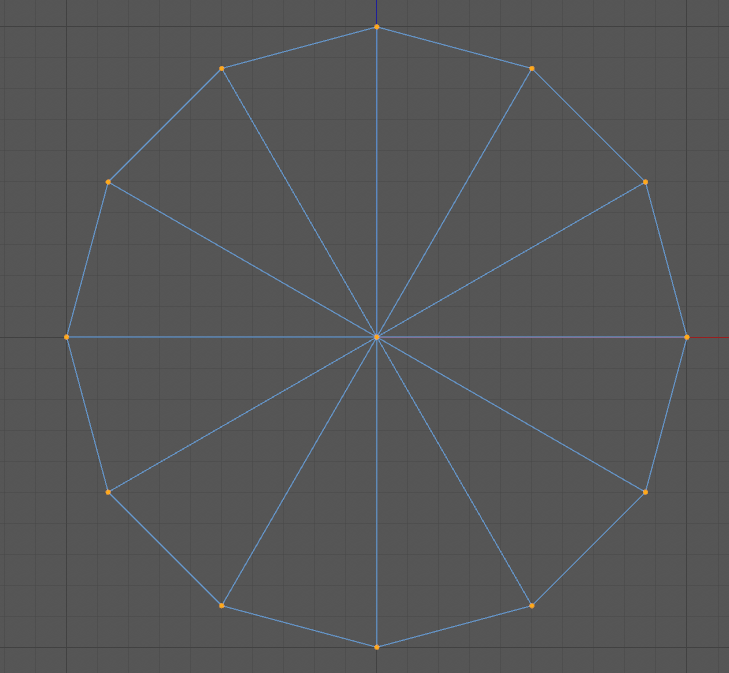
\includegraphics[width=\textwidth/6]{bilder/k12kreis.png} \\
	\end{figure} \\
	Die Triangle-Fans werden nun für die Löcher und Kugeln an den Positionen auf dem Spielfeld plaziert.
	\begin{figure}[h]
		\caption{Spielfeld ohne Texturen, mit k=64 für Triangle-Fans}
			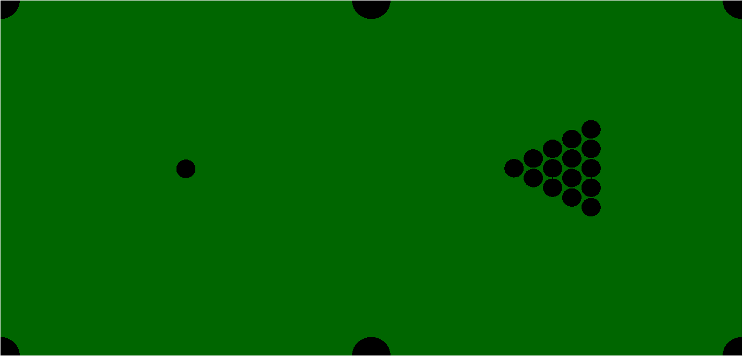
\includegraphics[width=\textwidth]{bilder/untextured_pool_low.png} 
	\end{figure}

\subsection{Texturierung}
	Die Farben für das Spielfeld sind trivial. 
	Die Kugeln hingegen müssen vom Spieler unterschieden werden können. 
	Wir müssen also Texturen auf Kreise abbilden. \\
	\begin{figure}[h]
		\caption{Billiardkugel Textur}
			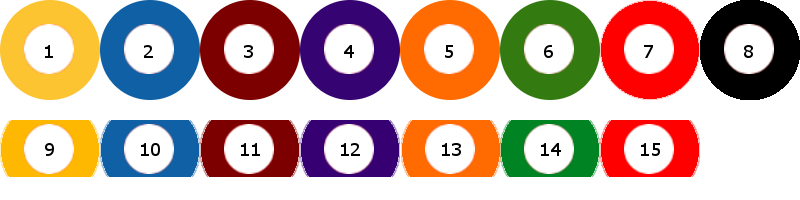
\includegraphics[width=\textwidth]{bilder/Balls.png} \\
	\end{figure} \\
	Um die Textur auf unsere Kugeln abzubilden verwenden wir u/v-Koordinaten. 
	Unsere Textur besitzt auf der $u$ und $v$ Achse einen Wertebereich von 0 bis 1. 
	Dabei ist $(0,0)$  oben links und $(1,1)$  unten rechts. 
	Jeder Kugel muss nun ein Ausschnitt der Textur zugewiesen werden. 
	Dafür bekommt jede Farbe einen Wert c.
	\begin{equation}\label{eq:color}
	c(b) = 
	\begin{cases}
		0, & \text{falls b Gelb} \\
		1, & \text{falls b Blau} \\
		2, & \text{falls b Rot} \\
		3, & \text{falls b Lila} \\
		4, & \text{falls b Orange} \\
		5, & \text{falls b Grün} \\
		6, & \text{falls b Rot} \\
		7, & \text{falls b Schwarz oder Weiß}
	\end{cases}
	\end{equation} 
	Außerdem bekommt jede Kugel einen Wert für die Fülle, wobei Voll = 0 ist und Halb = 1.  \\
	\begin{equation} \label{eq:full}
	f(b) = 
	\begin{cases}
		0, & \text{falls Kugel voll} \\
		1, & \text{falls Kugel halb}	
	\end{cases}
	\end{equation}\\
	\begin{figure}[h]
		\caption{Textur mit u/v-Koordinaten}
		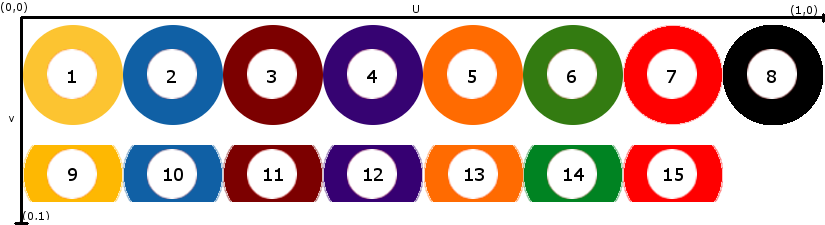
\includegraphics[width=\textwidth]{bilder/ballsachsen}
	\end{figure} \\
	Nun können wir uns eine Funktion erstellen, die anhand von Farbe und Fülle die Textur ausschneidet und auf die Kugel abbildet. 
	Dazu berechnen wir zuallererst die Anfangsposition der Textur. 
	Diese setzt sich zusammen aus der Farbe c und der Fülle f. \\
	Vorgedanke: Der Durchmesser einer Kugel auf unserer Textur ist $\frac{1}{8}$ für $u$, weil es 8 Kugeln pro Reihe gibt und die u Koordinate genau 1 lang ist. Der Durchmesser auf der $v$-Achse hingegen ist $\frac{1}{2}$, weil es nur 2 Reihen gibt und die Textur trotzdem 1 lang ist. \\
	Mittelpunkt m der Textur: \\
	\begin{equation}\label{eq:texStart}
	\begin{aligned} 
		x(b) = \frac{1}{16} + \frac{1}{8} \cdot c(b), c(b) = \text{Farbe der Kugel \eqref{eq:color}} \\
		y(b) = \frac{1}{4} + \frac{1}{2} \cdot f(b), f(b) = \text{Fülle der Kugel \eqref{eq:full}}
	\end{aligned}
	\end{equation}
	Nun fehlen noch die Texturkoordinaten für den Kreis um den Mittelpunkt der Textur herum.
	Die Berechnung läuft dabei analog zum Triangle-Fan mit dem Unterschied in der Skalierung und Startposition. 
	So benutzen wir nicht den Radius der Kugeln des Spiels, sondern die Größe der Kugel auf der Textur und als Startpunkt unser vorher berechnetes x und y in \eqref{eq:texStart}. 
	\begin{equation}\label{eq:texXY}
	\begin{aligned}
		 xTex(b) =  x(b) + \cos(\delta \cdot i) \cdot \frac{1}{16}, \\
		 yTex(b) =  y(b) + \sin(\delta \cdot i) \cdot \frac{1}{4}, \\
		\text{mit } \delta \text{ nach }\eqref{eq:delta} \text{ und } i \text{ nach } \eqref{eq:circleCoord}
	\end{aligned}
	\end{equation}
	Die Textur wird dann beim erstellen des Triangle-Fans auf die Dreiecke gezeichnet. Dabei bekommen die Dreiecke für den Mittelpunkt $(x,y)$ als Texturkoordinaten \eqref{eq:texStart} und der Punkt auf dem Umriss bekommt dann $(xTex,yTex)$ \eqref{eq:texXY}.
\subsection{Kollisionsberechnung}
	Die Kollisionsberechnung lässt sich aufteilen in 3 Bereiche: \begin{itemize}
		\item [1.] Kollision von Kugeln mit Wand und Löchern
		\item [2.] Kollision von Kugeln mit anderen Kugeln
		\item [3.] Kollision der Weißen Kugel mit dem Queue (Kapitel 3.3.3)
	\end{itemize}
	\subsubsection{Kollision von Kugeln mit Wand und Löchern}
		Das Kollidieren mit den Wänden ist sehr simpel: Wir geben  unsere Breite und Höhe des Spielfeldes als Grenzen an. Wenn die Kugel zu nah an eine der Wände kommt wird ihre Geschwindigkeit umgekehrt. Dementsprechend machen wir eine Fallunterscheidung mit 4 Fällen für die 4 verschiedenen Wände: \begin{itemize}
			\item [1.] Die Linke Wand (x=0)
			\item [2.] Die Rechte Wand (x=w)
			\item [3.] Die Obere Wand (y=0)
			\item [4.] Die untere Wand (y=h)
		\end{itemize}
		Dabei gilt $ h = $ Höhe des Spielfeldes, $ w = $ Breite des Spielfeldes und $l = $ Radius der Löcher.
		Die Änderung der Geschwindigkeit ist dann:
		\begin{equation}
		vy = \begin{cases}
			-vy, & \text{ falls } y \leq (h- l) \land y \geq l\\
			vy, & sonst 
		\end{cases}
		\end{equation}
		Das gilt für Fall 1 und 2. Für Fall 3 und 4 benötigen wir noch eine Bedingung mehr:
		 \begin{equation}
		vx = \begin{cases}
		-vx, & \text{ falls } (x \leq (w/2 - l) \land x \geq l) \lor (x \geq (w/2 + l) \land (x \leq (w- l) \\
		vx, & sonst 
		\end{cases}
		\end{equation}
		Wir überprüfen also, ob die Kugel eine der Beiden Strecken zwischen den Löchern trifft, wenn sie vorher den Rand des Spielfeldes erreicht hat. 
	\subsubsection{Kollision mit anderen Kugeln}
		Die Kollisionsberechnung für 2 Kugeln war uns bereits vorgegeben aus einem Beispiel für ein AirHockey Spiel. 
		Der Unterschied liegt darin, dass im Airhockey nur eine Kugel durch die Kollision ihre Geschwindigkeit ändert. Die beiden Schläger werden durch die Kollision nicht verändert. \\  
		Wir nehmen nun eine Kugel und berechnen mit der Methode alle Kollisionen mit anderen Kugeln, indem wir statt dem Schläger die jeweils andere Kugel einsetzen. Das muss für jede Kugel einmal ausgeführt werden.  \\
		
		%\begin{equation}
		%d = \sqrt{(x_2 - x_1)^2 + (y_2-y_1)^2} 
		%\end{equation}
		%Wenn diese Distanz kleiner ist als der Durchmesser $r*2$ einer Kugel, dann gibt es eine Kollision. \\
%		Die Kollision wird ausgewertet, indem zunächst die Normale berechnet wird: 
%		\begin{equation}
%		\begin{aligned}
%		nx = x_1 - x_2; \\
%		ny = y_1 - y_2; \\
%		\end{aligned}
%		\end{equation}
%		Das Ergebnis $(nx,ny)$  wird dann noch normalisiert. Dann berechnen wir die Tangente dazu:
%		\begin{equation}
%		\begin{aligned}
%		tx = -ny \\
%		ty = nx
%		\end{aligned}
%		\end{equation}
%		Als nächstes wird die Relative Geschwindigkeit zwischen beiden Kugeln berechnet. Dabei bezeichnen wir die Geschwindigkeit einer Kugel als vx bzw. vy (also $vx_1$ für die Geschwindigkeit auf der X-Achse der Kugel $b_1$).
%		\begin{equation}
%		\begin{aligned}
%		vrx = vx_2 - vx_1 \\
%		vry = vy_2 - vy_1
%		\end{aligned}
%		\end{equation}

	\subsubsection{Zusammenfassung}
		 Nun haben wir ein Spielfeld mit Texturierten Kugeln die miteinander kollidieren.
		 \begin{figure}[h]
		 	\caption{Fertiges Spielfeld}
		 	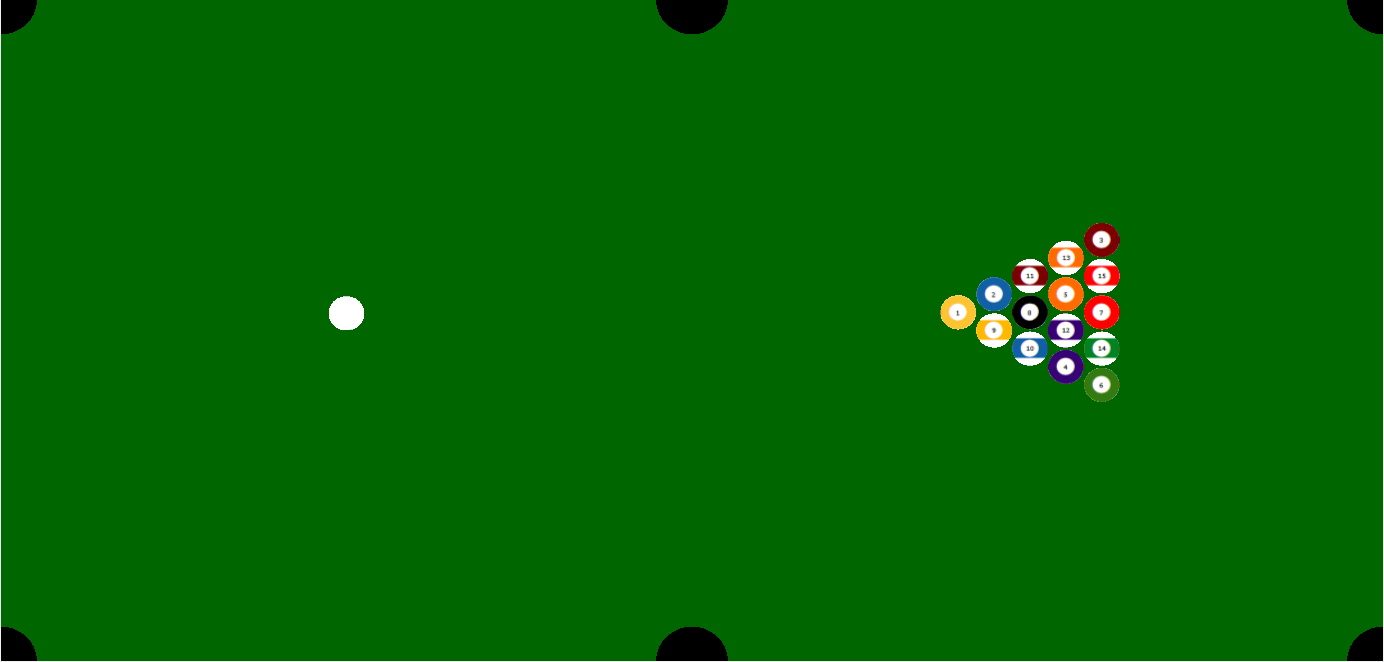
\includegraphics[width=\textwidth]{bilder/Spielfeld.png}
		 \end{figure}


\section{Kamerakalibrierung}
%Um einen Punkt, welcher von der Kamera bzw. der Queue-Erkennung erfasst wurde, korrekt in das Spielfeld zu projezieren, müssen folgende Schritte durchlaufen werden:\\
%Der gegebene Punkt, welcher in einem 2D Vektor vorliegt, muss in das gegebene Spielfeldkorrdinatensystem transformiert werden. Hierfür muss das Spielfeld zunächst von der Kamera erkannt werden um anschließend im Kamerakoordinatensystem festgehalten zu werden. Da das Kamerabild eine natürliche Verzerrung des Bildes beinhaltet, muss ebenso diese Verzerrung entzerrt werden. Dies wird mit Hilfe eines bekannten Musters, welches in diesem Projekt ein Schachbrettmuster ist, bewerkstelligt, in welchem signifikante Eckpunkte erkannt, daraus die Verzerrung ermittelt und entzerrt werden. Nachdem dies erfolgt ist, kann ein erkannter und entzerrter Punkt aus der Kamera in das Spielfeldkoordinatensystem übertragen werden. Hierfür muss eine Umrechnung erfolgen, da das Kamerakoordinatensystem oben links den (0,0)-Punkt hat und das Spielfeld unten rechts.

%\subsection{Einleitung}
%Sobald die Anwendung gestartet wird, wird die Kamera verbunden und ein Timer fragt alle 16ms ab, ob die Kalibrierung gestartet werden soll. Wenn dem so ist, wird auf dem Spielfeldbereich ein Schachbrettmuster gerendert und nach jedem Ablauf des Timers, hier dem entsprechend alle 16ms, Fotos aufgenommen. Sobald eine festgelegte Grenze von aufgenommenen Fotos erreicht wurde, werden diese ausgewertet, ob das Schachbrettmuster auf diesen Fotos erkannt wurde. Falls dem nicht so ist, werden erneut Fotos aufgenommen. Ansonsten werden die Eckpunktkoordinaten des erkannten Musters gespeichert und damit die Entzerrung ausgeführt. Im Anschluss kann ein, von der Queue-Erkennung erfasster Punkt, entzerrt und ins Spielfeld übertragen werden.

\subsection{Darstellung des Erkennungsmusters}
Um die Kamera kalibrieren und das Kamerabild entzerren zu können, muss die Kamera ein bekanntes Erkennungsmuster finden und in diesem bestimmte Eckpunkte erfassen und auswerten können. In unserem Projekt wird ein Schachbrettmuster genutzt, von welchem die inneren Eckpunkte erkannt werden. Hierfür muss die Anzahl der Kacheln in der Horizontalen = $Hor$, sowie in der Vertikalen = $Vert$, bekannt bzw. festgelegt sein, um für jede Kachel die selbe Höhe und Breite zu haben und trotzdem die gesamte Höhe und Breite des Spielfeldes abzudecken. Die Höhe und Breite wird wie folgt berechnet:\\
$Hoehe_{Kachel} = \frac{Hoehe_{Game}}{Vert}$, $Breite_{Kachel} = \frac{Breite_{Game}}{Hor}$\\
Nun wird für jedes $i \in [1,Hor]$ alle $j \in [1,Vert]$ eine Kachel gerendert mit den Koordinaten oben links ($i \cdot Hoehe_{Kachel}$, $j \cdot Breite_{Kachel}$) und den Koordinaten unten rechts ($(i+1) \cdot Hoehe_{Kachel}$, $(j+1) \cdot Breite_{Kachel}$). Zudem wird bei jeder neuen Kachel in der Horizontalen die invertierte Farbe der vorherigen Kachel als Grundfarbe gewählt und in der Vertikalen für die erste Kachel die invertiere Farbe der darüber liegenden Kachel gewählt, damit das klassische Schwarz-Weiß-Muster eines Schachbretts visualisiert wird.
\begin{figure}[h]
	\label{fig:chessboard}
	\centering
	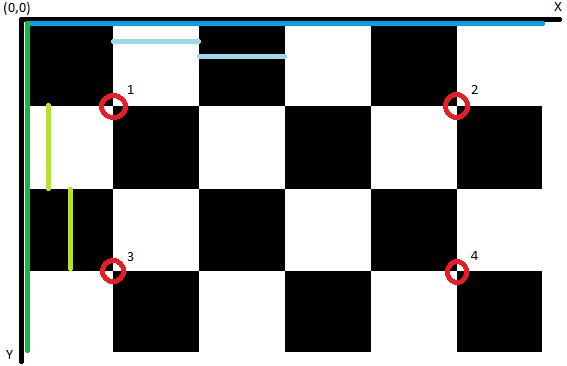
\includegraphics[scale=0.8]{bilder/schachbrett.png}
	\caption{Schachbrettmuster rendern}
\end{figure}

\subsection{Entzerrung des Kamerabildes/Punktes}
%Bildkoordinaten = BK, Weltkoordinaten = WK, Patterneckpunkte = PE, Vector 2/3 Point = 2/3V\\
%Nimmt 20 Fotos auf und wertet diese dann in der $Calibration$ aus:\\
%$patternWorldCoordinates$ = 3V mit $(x*a,y*a,0)$ für alle $x \in Hor-1$ für alle $y \in Vert-1$ und $a$ = Kantenlänge für Kachel in WK\\
%$patternCorners$ = 2V Speicher für PE in BK\\
%$patternWorldBuffer$ = 3V Speicher für PE in WK\\
%$pointBuffer$ = 2V Zwischenspeicher für PE in BK (wird für jedes Bild neu initialisiert)\\

\subsection{Punktübertragung von Kamera in Spiel}
Der letzte Abschnitt der Kamerakalibierung stellt das Übertragen eines von der Queue-Erkennung gegebenen Punktes, welcher sich im Kamerakoordinatensystem befindet, in das Spielfeldkoordinatensystem um diesen dann in den Spielmechanismus als Queueposition einzubinden.
Um dies einwandfrei zu ermöglichen, müssen die äußersten Eckpunkte des, von der Kamera erfassten, Schachbrettmusters im Kamerakoordinatensystem bekannt sein. Da allerdings nur die Eckpunkte auf der Innenseite des äußersten Ringes des Schachbretts erkannt werden, müssen die ganz äußersten Eckpunkte wie folgt berechnet werden:\\
$Lila_{min} = Gruen_{min} - Rot_{min}$\\
$Lila_{max} = Rot_{max} - Gruen_{max}$
\begin{figure}[h]
	\label{fig:chessboard}
	\centering
	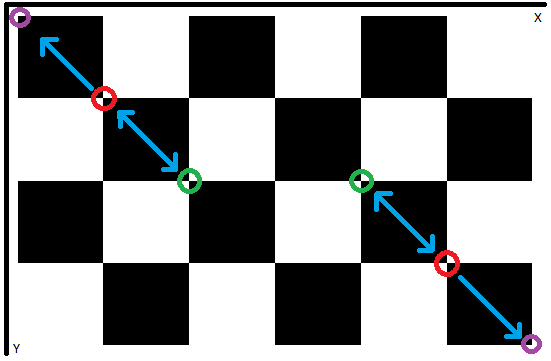
\includegraphics[scale=0.8]{bilder/schachbrettdiff.png}
	\caption{Schachbrettmuster Eckpunkte}
\end{figure}\\
Nun sind die äußersten Eckpunkte des Spielfeldes im Kamerakoordinatensystem bekannt und es ist möglich einen beliebigen 2D Punkt in das Spiel zu projezieren. Hier wird unter zwei Fällen unterschieden. Entweder liegt der übergebene Punkt der Kamera im Spielbereich oder nicht: $X \in [x_{min}, x_{max}]$ und $Y \in [y_{min},y_{max}]$.
Sofern dieser Punkt im Spielbereich liegt, wird dieser Punkt $P$ in das Spielkoordinatensystem projeziert, was wie folgt berechnet wird:\\
$X = \dfrac{(P.x - MIN.x) * UR}{(MAX.x - MIN.x)}$, 
$Y = \dfrac{(MAX.y - P.y) * OL}{(MAX.y - MIN.y)}$
\begin{figure}[h]
	\label{fig:chessboard}
	\centering
	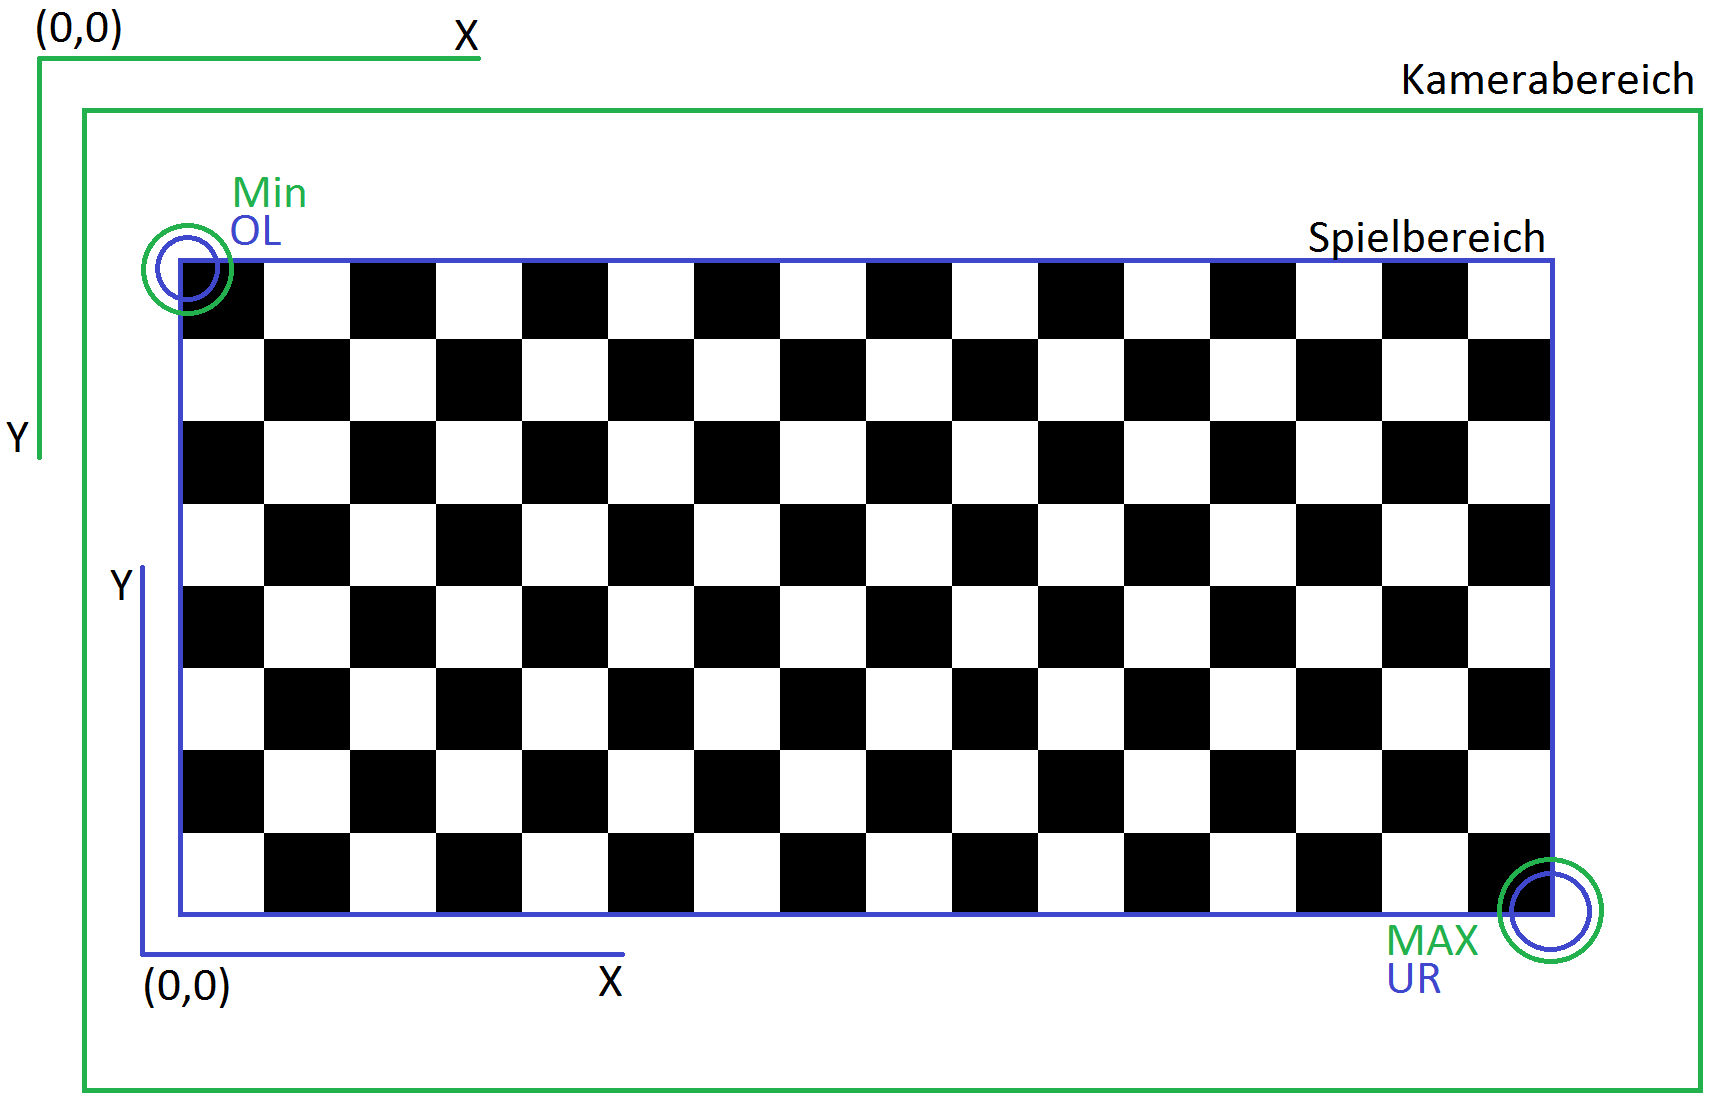
\includegraphics[scale=0.3]{bilder/schachbrettkamera.png}
	\caption{Kamera- und Spielkoordinatensystem}
\end{figure}\\

\section{Queue-Detektion}

Wie schon zuvor erläutert, soll es dem Spieler möglich sein, mit dem realen Queue die simulierten Kugeln zu stoßen.
Dazu wird das Spielfeld von einer Kamera erfasst. 
Um die Interaktion des Queues mit den Kugeln zu ermöglichen, müssen in dem Eingabebild der Kamera die für die Kollisionsberechnung relevanten Punkte des Queues extrahiert werden.

In den folgenden Abschnitten wird dazu eine Möglichkeit beschrieben, welche zunächst mittels eines Schwellwertverfahrens den Queue vom Hintergrund segmentiert.
Basierend auf dem segmentierten Bild werden dann unter Verwendung der Hauptkomponentenanalyse zwei Kollisionspunkte ermittelt.
Schließlich wird die Einbindung der Kollisionspunkte in die Kollisionsberechnung erläutert, welche die Detektion des Queues abschließt.

\subsection{Segmentierung}
Sei $\textbf{I} \in \{0, \dots, 255\}^{b \times h \times 3}$ das von der Kamera aufgenommene $b \times h$ große RGB-Farbbild.
Ziel der Segmentierung ist es, ein Binärbild $\textbf{B} \in \{0,1\}^{b \times h}$ zu erzeugen, welches die Pixel im Eingabebild charakterisiert, die dem Queue zugeordnet werden.

Da der Queue mit einer schwarzen Farbe lackiert wurde, wird dies mithilfe eines Schwellwertverfahrens basierend auf dem Farbwert der Pixel bewerktstelligt.
Das im RGB-Farbraum vorliegende Eingabebild $\textbf{I}$ wird dazu zunächst in den HSV-Farbraum überführt. 
Im HSV-Farbraum wird ein Farbwert durch seinem Farbton $H \in [0, 360]$, der Sättigung $S \in [0, 1]$ und dem Helligkeitswert $V \in [0, 1]$ dargestellt.

\begin{figure}[H]
	\label{fig:HSVRGB}
	\subfigure[]{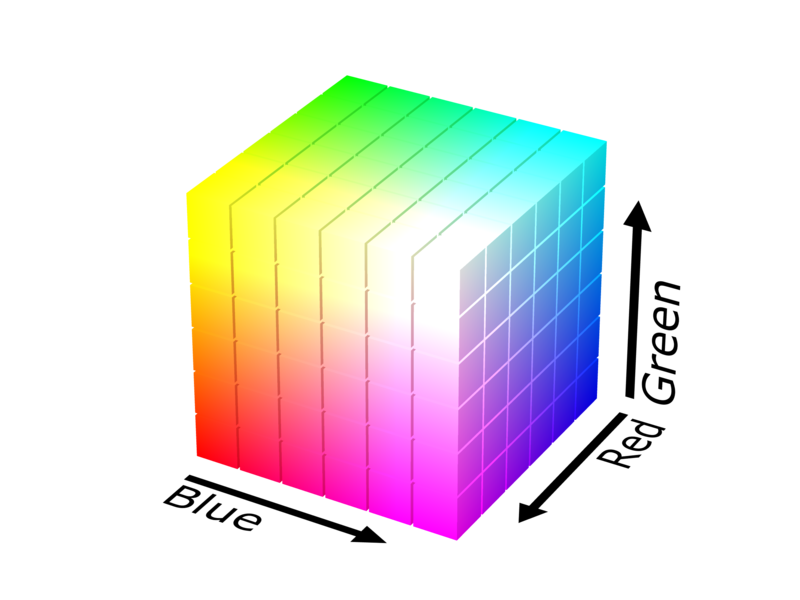
\includegraphics[height=3.3cm]{bilder/rgb.png}\label{fig:RGB}}
	\subfigure[]{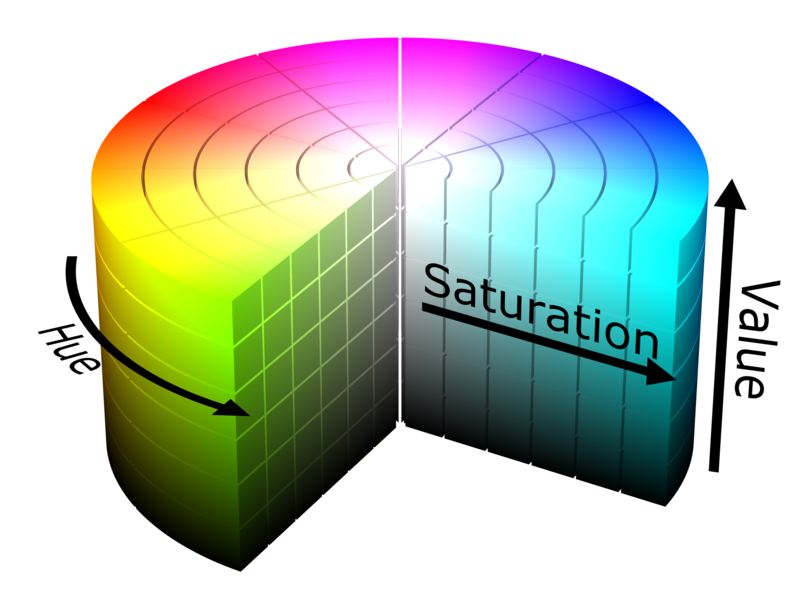
\includegraphics[height=3.0cm]{bilder/hsv.png}\label{fig:HSV}}
	\centering
	\caption{Darstellung von Farbtönen im (a) RGB-Farbraum \cite{RGBCube} durch Rot-, Grün- und Blauanteil, und im (b) HSV-Farbraum \cite{HSVCylinder} durch Farbton (Hue), Sättigung (Saturation) und Helilgkeitswert (Value). Dunkle Farben im HSV-Farbraum haben einen kleinen Helligkeitswert.}
\end{figure}

Somit kann allein durch einen Schwellwert $\theta$ für den Helligkeitswert der schwarze Queue vom Rest des Bildes segmentiert werden.
Für das transformierte Bild $\textbf{I}_{HSV}$ ergibt sich die Berechnung des Wertes von $\textbf{B}$ an der Stelle $i, j$ für einen Schwellwert $\theta$ somit durch folgende Formel:
\begin{equation*}
\textbf{B}[i,j] = \begin{cases}
1 &\text{, falls $\textbf{I}_{HSV}[i, j, 3] \leq \theta$}\\
0 &\text{sonst}
\end{cases}
\end{equation*}

Durch die unterschiedliche Beleuchtung des Queues ergeben sich in dem entstehenden Binärbild größere Lücken, die die weitere Erkennung des Queues beeinflussen würden.
Um dies zu verhindern werden diese durch die Anwendung eines morphologischen Closings gefüllt.
Bei einem morphologischen Closing wird zunächst eine Dilatation und daraufhin eine Erosion auf dem Bild mit einem $k \times k$ großen, ellipsoiden Fenster durchgeführt. 
Für die Dilatation wird mit dem Fenster über das Bild gelaufen und dabei der zentrale Pixel des Fensters auf den maximalen Wert im Fenster gesetzt.
Analog dazu wird bei der Erosion der Wert des zentralen Pixels auf den minimalen Wert im Fenster gesetzt.
Insgesamt werden durch diese beiden Operationen die Lücken im Binärbild geschlossen ohne die Kontur des Queues zu vergrößern.

\begin{figure}[H]
	\label{fig:thresholded}
	\subfigure[]{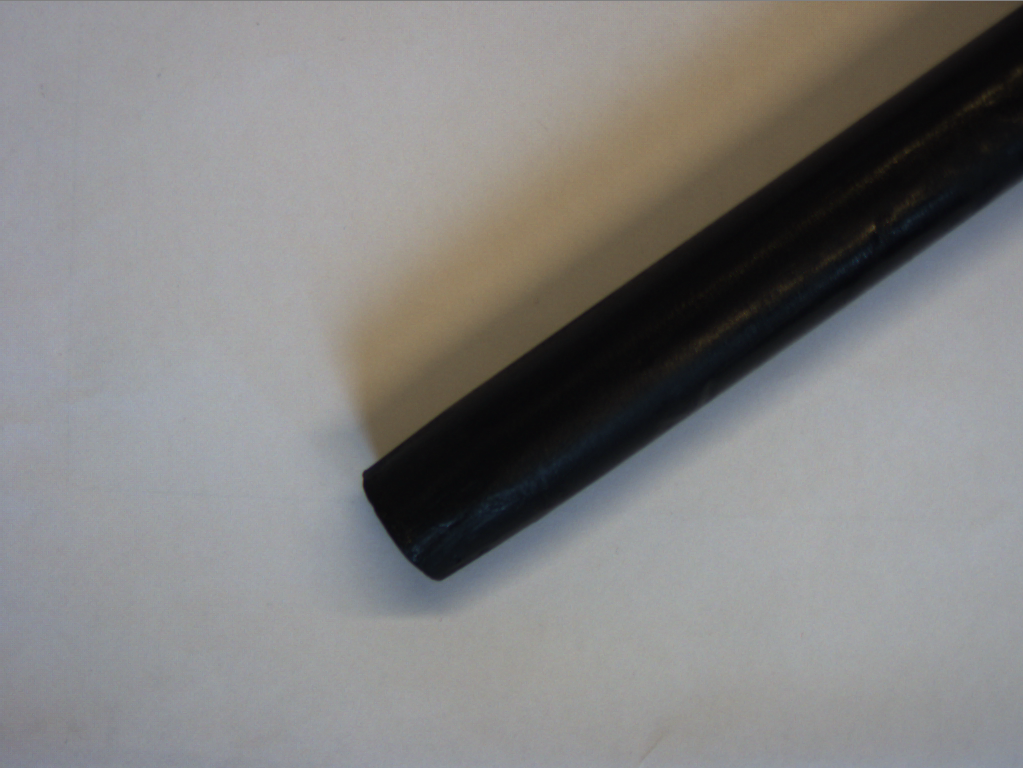
\includegraphics[height=3.3cm]{bilder/queue_orig.png}}
	\subfigure[]{
\includegraphics[height=3.3cm]{bilder/queue_thresholded.png}}
	\subfigure[]{
\includegraphics[height=3.3cm]{bilder/queue_close.png}}	
	\centering
	\caption{Ergebnis der Segmentierung des Eingabebildes. (a) Eingebild mit $1024 \times 768$ Pixeln, (b) Binärbild aus Schwellwertverfahren ($\theta = 30$),  (c) Ergebnis des morphologischen Closings ($k=9$)}
\end{figure}

\subsection{Erkennung der Queue-Enden}
Um nicht mit jedem im Binärbild als Queue klassifizierten Punkt kollidieren zu müssen wird nur mit den Enden des Queues kollidiert.
Zur Berechnung der Position der beiden Enden wird zunächst mittels der Hauptkomponentenanalyse \cite{OpenCV:PCA} die Hauptachse des Queues im Bild bestimmt. 
Dazu werden die Koordinaten $i, j$ der Punkte aus $\textbf{B}$ mit $\textbf{B}[i,j] = 1$ als Zeilenvektoren in einer $n \times 2$ Matrix $\textbf{X}$ zusammengeführt.
Daraufhin wird der Mittelpunkt \textbf{c} der $n$ Punkte sowie die Abweichung $\textbf{A}$ zu dem Mittelpunkt berechnet:
\begin{equation*}
\textbf{c}[j] = \frac{1}{n}\sum_{i=1}^{n}\textbf{X}[i, j]\text{ mit }j = 1, 2
\end{equation*}
\begin{equation*}
\textbf{A} = \textbf{X} - \textbf{h}\textbf{c}^T \text{ mit } \textbf{h}[i] = 1 \text{ für } i=1,\dots,n
\end{equation*}

Aus der Matrix \textbf{A} lässt sich nun die $2 \times 2$ empirische Kovarianzmatrix $\textbf{C}$ berechnen:
\begin{equation*}
	\textbf{C} = \frac{1}{n-1}\textbf{A}^{T}\textbf{A}
\end{equation*}
Schließlich werden die zwei Eigenvektoren und Eigenwerte von $\textbf{V}$ bestimmt. 
Da der Eigenvektor $\textbf{e}$, dem der größere Eigenwert $\lambda_e$ zugeordnet ist, in die Richtung der größten Varianz der Punkte zeigt, ist die gesuchte Hauptachse gegeben durch $\textbf{x}(t) = t \cdot \textbf{e} + \textbf{c}$.

Um nun die Endpunkte des Queues zu bestimmen, müssen alle Punkte auf die zuvor bestimmente Hauptachse projiziert werden.
Für einen Punkt $\textbf{x} = (i, j)$ mit $\textbf{B}[i,j] = 1$ ergeben sich die neuen Koordinaten $\textbf{x}'$ durch
\begin{equation*}
	\textbf{x}' = s \cdot \textbf{e} + \textbf{c}\text{ mit } s = \frac{\textbf{e} * (\textbf{x} - \textbf{c})}{||\textbf{e}||}
\end{equation*}
Dabei bezeichnet $*$ das Skalarprodukt zweier Vektoren sowie $||\cdot||$ die euklidische Norm eines Vektors.
Die beiden Punkte, die am weitesten von dem Mittelpunkt \textbf{c} entfernt sind, sind die beiden Enden des Queues. Für diese Punkte $\textbf{x}_1'$, $\textbf{x}_2'$ ist $s$ entweder minimal oder maximal. 

\begin{figure}[H]
	\label{fig:pca}
	\subfigure[]{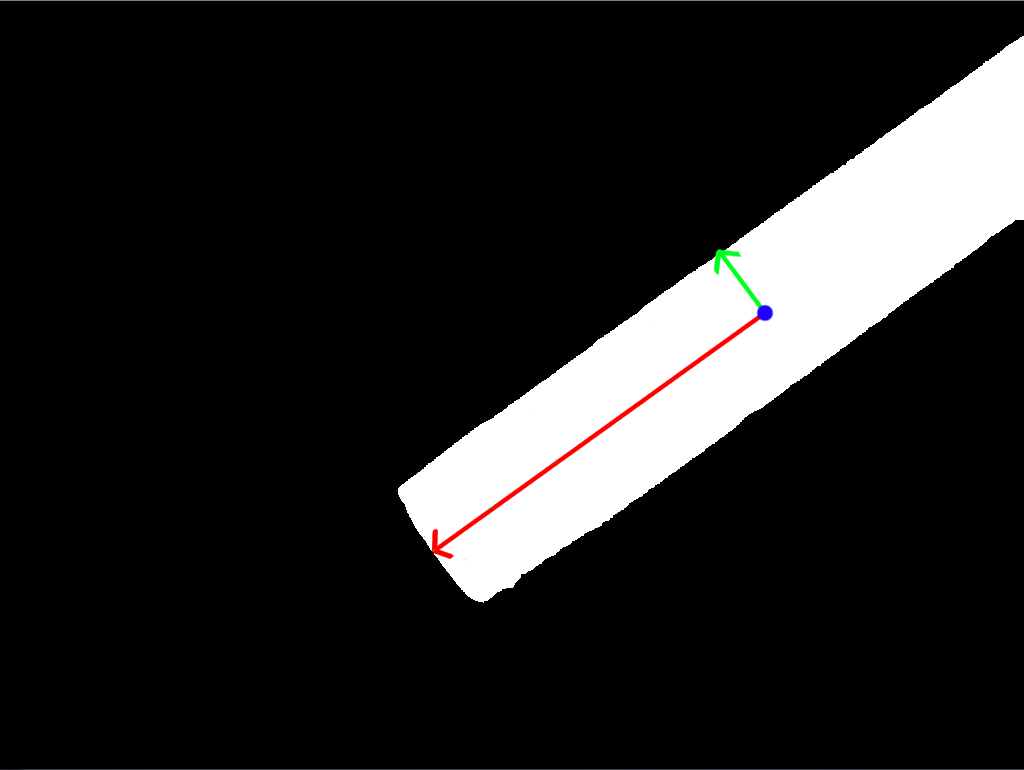
\includegraphics[height=4cm]{bilder/queue_pca_1.png}}
	\subfigure[]{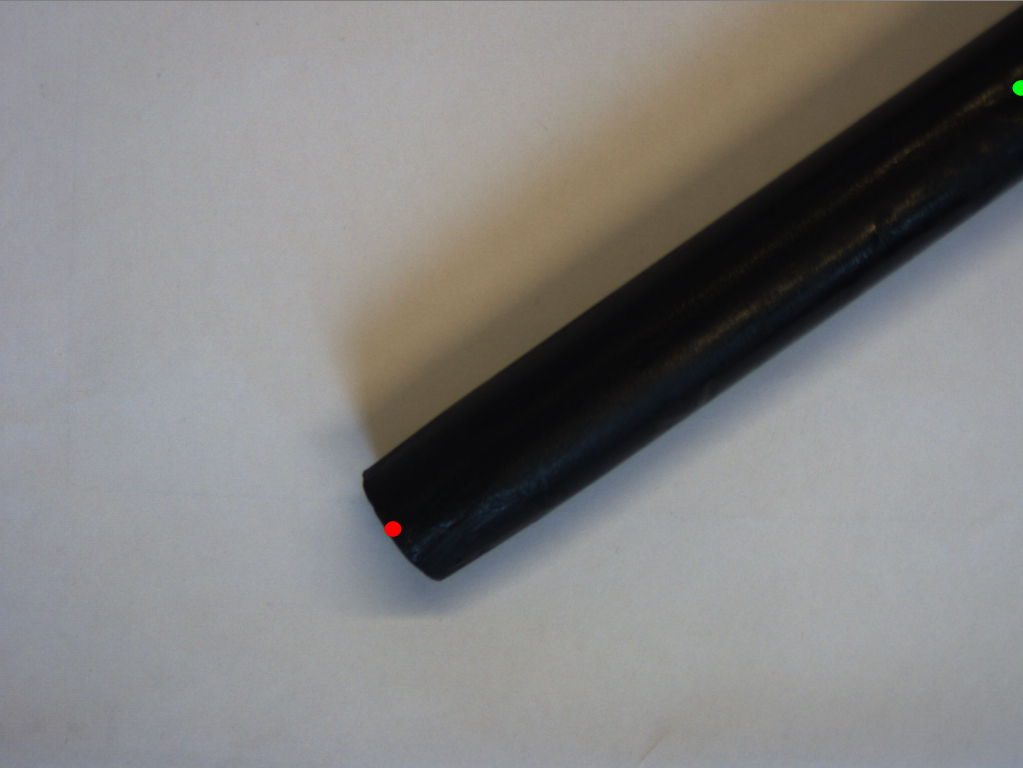
\includegraphics[height=4cm]{bilder/queue_pca_2.png}}
	\centering
	\caption{Erkannte Endpunkte des Queues. (a) Binärbild mit Zentrum \textbf{c} in blau sowie die berechneten Eigenvektoren in rot und grün, (b) Originalbild mit erkannten Endpunkten des Queues}
\end{figure}


Da das Vorzeichen für $s$ sich in aufeinanderfolgenden Bildern verändern kann, müssen die Punkte für die Kollisionsberechnung korrekt ihrem Vorgänger zugeordnet werden.
Dies wird bewerkstelligt, indem ein Punkt dem näheren der beiden Vorgänger-Punkte zugeordnet wird.
Weiterhin kann keines der beiden Enden mit Sicherheit als Spitze des Queues klassifiziert werden.
Daher wird die Kollisionsbehandlung mit beiden Enden ausgeführt.
Dies hat auf den Spielfluss jedoch keine Auswirkungen, da eines der Enden meist am Rand des Spielfeldes ist.

\subsection{Kollisionserkennung}

Bei Stoßbewegungen mit dem Billard-Queue kann es zu hohen Geschwindigkeiten der Queue-Enden kommen. 
Da die Kamera mit einer Wiederholfrequenz von 25 Bildern pro Sekunde Bildaufnahmen macht, kann es passieren, dass ein Ende sich zu schnell bewegt und über eine Kugel hinwegspringt ohne ein Kollision auszulösen. 
Daher kann die Kollisionsüberprüfung nicht nur auf der aktuellen Position des Queue-Endes basieren.
Stattdessen wird der Kollisionspunkt durch das Schneiden der Kugel und einem  Liniensegment berechnet. 
Das Liniensegment ergibt sich dabei durch die aktuelle Position und der voherigen Position der Queue-Enden.

Die Schnittpunkte einer Kugel mit Mittelpunkt $\textbf{c}$ und Radius $r$ und einem Liniensegment mit Startpunkt  $\textbf{x}^{(t-1)}$ und Endpunkt $\textbf{x}^{(t)}$ lässt sich wie folgt berechnen:

\hspace{-1cm}\begin{minipage}{.333333\linewidth}
	\begin{equation*}
	\textbf{d} = \textbf{x}^{(t)} - \textbf{x}^{(t-1)}
	\end{equation*}
\end{minipage}%
\begin{minipage}{.333333\linewidth}
	\begin{equation*}
	\textbf{f} = \textbf{x}^{(t-1)} - \textbf{c}
	\end{equation*}
\end{minipage}
\begin{minipage}{.333333\linewidth}
	\begin{equation*}
	s_{1,2} = \frac{-2 \cdot (\textbf{d} * \textbf{f}) \pm \sqrt{||\textbf{f}||^2 - r^2}}{2 \cdot ||\textbf{d}||^2}
	\end{equation*}
\end{minipage}
\vspace{0.3cm}

Falls $s_1 \in [0, 1] \subset \mathbb{R}$ ist, so ist der Schnittpunkt durch $\textbf{x}_c = s_1 \cdot d + \textbf{x}^{(t-1)}$ gegeben. 
Mit diesem wird dann die übliche Kollisionsberechnung durchgeführt.
In den anderen Fällen darf keine Kollision ausgeführt werden, da entweder kein Schnittpunkt exisiert oder der Schnittpunkt kein gültiger Kollisionspunkt wäre:

\begin{figure}[H]
	\label{fig:collision}
	\subfigure[]{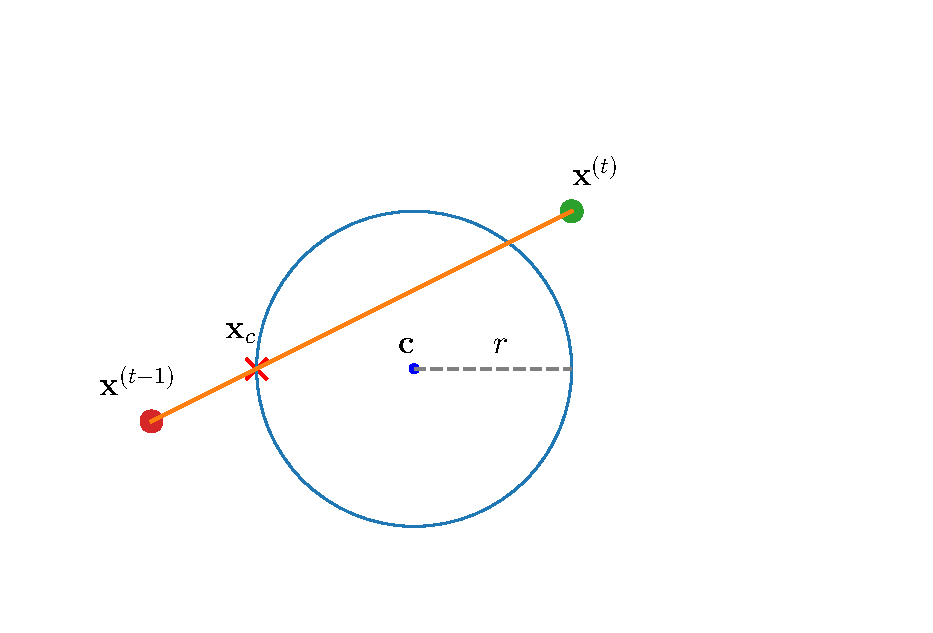
\includegraphics[height=4cm]{bilder/hit.eps}}
	\hspace{-1.8cm}
	\subfigure[]{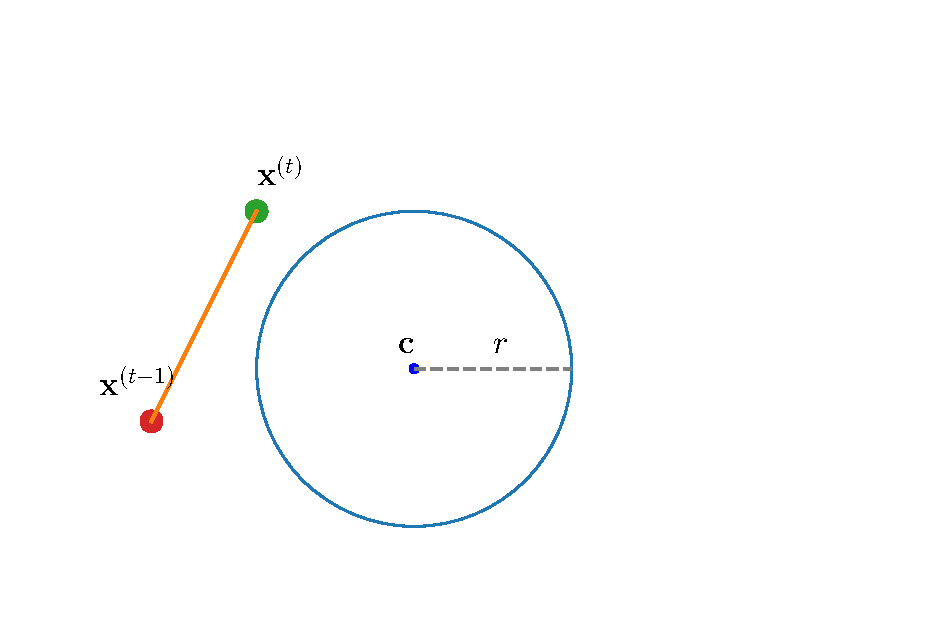
\includegraphics[height=4cm]{bilder/nohit.eps}}	\hspace{-2.4cm}
	\subfigure[]{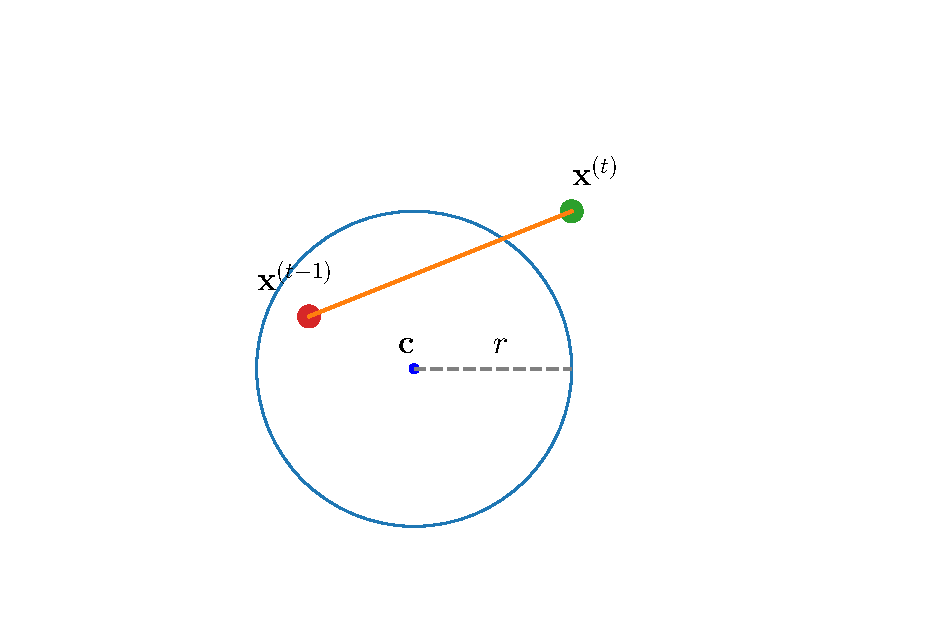
\includegraphics[height=4cm]{bilder/exitwound.eps}}
	\centering
	\caption{Unterschiedliche Fälle bei der Kollisionserkennung.
	(a) Kollision in $\textbf{x}_c$, (b) Keine Kollision, (c) Kollision mit Schnittpunkt wäre fehlerhaft}
\end{figure}


\section{Spielregeln und Benutzerinteraktion}
Damit die Benutzerinteraktion funktioniert, müssen zunächst die Spielregeln ins Spiel eingebunden werden. Das Spiel das 8er- Ball-Billiard: \\
 8er Ball wird mit einem Spielball (weiss) und 15 nummerierten farbigen Kugeln gespielt. 14 der farbigen Kugeln werden in zwei Gruppen eingeteilt. Nr. 1 bis 7 sind vollfarbige (volle) Kugeln. Nr.9 bis 15 sind gestreiftfarbige (halbe) Kugeln. Zu Beginn werden alle 15 farbigen Bälle mit dem Dreieck so aufgestellt, dass die vorderste Kugel des Dreiecks auf dem Fusspunkt zu liegen kommt. Ziel des Spieles ist es, zuerst eine Serie von vollen oder halben Bällen und zuletzt den 8er Ball in die Löchern zu versenken. Jeweils der Gewinner eines Spieles eröffnet das nächste Spiel( Alternativ kann auch abwechslungsweise angespielt werden).

\subsection{Spielregeln}
Sobald der erste Spieler seinen Zug gemacht hat, started das Spiel.
Sollte der Spieler einen Ball eingelocht haben, überprüft die Spiellogik, ob es sich hierbei um eine vollen Ball handelt oder halben Ball. Entsprechend wird dabei der Balltyp des Spielers auf 'True' für einen vollen Ball oder auf 'False' für einen halben Ball gesetzt. Anschließend darf der derzeitig aktuelle Spieler einen weiteren Zug machen. \begin{equation}
BallTyp = \begin{cases}
True, & \text{ Für Volle Kugel } \\
False, & \text{ Für Halbe Kugel }
\end{cases}
\end{equation}

\begin{equation}
currentPlayer = \begin{cases}
0, & \text{ Für Ersten Spieler } \\
1, & \text{ Für Zweiten Spieler }
\end{cases}
\end{equation}

Hat der Spieler den Ball nicht eingelocht, dann wird der Spieler gewechselt.

dabei wird der BallType beim ersten spielzug nicht gesetzt, da niemand eine Farbe zugeordnet bekommen hat.
Um das Spiel zu Gewinnen muss man alle Kugeln eingelocht haben, die für den Spieler zugewiesen wurden. Die Letzte Kugel ist die Schwarze Kugel. Sollte diese versenkt worden sein, bevor alle Kugeln des Spielers versenkt sind, dann hat der Aktuelle Spieler entsprechen Verloren und ein Pop-up Fenster erscheint. Andernfalls hat Er  Gewonnen.

\subsection{Benutzerinteraktion}

Bevor ein Benutzer das Programm gestartet hat, müssen vorher einige voraussetzungen erfüllt werden. Das Programm benötigt zu ausführung eine Kamera. Diese wird zum Kalibrieren des Spielfeldes benötigt. Sollte die Kamera verbunden worden sein, so muss sie nun auf das Programm-Fenster zeigen. Zu Begin bei der Ausführung des Programms, wird ein Pop-up Fenster angezeigt, welche fragt ob die Kalibrierung gestartet werden kann(siehe Abbildung 3.6: Kalibrierung-Pop-up).
 \begin{figure}[h]
	\centering
	\caption{Kalibrierung-Pop-up}
	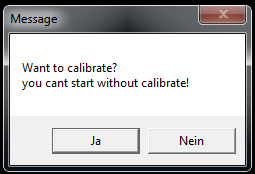
\includegraphics[width=\textwidth/3]{bilder/Calibrate-Popup.png}
\end{figure}\\
Mit dem Drücken des 'Ja'-Knopfes wird ein Signal richtung der Kamerakalibrierung geschickt und sie wird gestartet. Sollte 'Nein' gedrückt worden sein, so wird das Programm geschlosse, da das Programm die kalibrierung benötigt.
Nach der Kalibrierung wird ein weiteres Pop-up Fenster angezeigt, ob man das Spiel nun starten möchte. Wenn 'Ja' gedrückt wird, dann wird das ganze Spielfeld angezeigt. 
 \begin{figure}[h]
	\centering
	\caption{StartGame-Pop-up}
	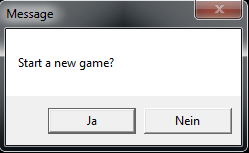
\includegraphics[width=\textwidth/3]{bilder/startGame-Popup.png}
\end{figure}\\
Nebenbei werden auch die Labels für den CurrentPlayer sowie des Balltypen angezeigt.
Das Spiel kann nun gespielt werden mit einem Queue. Hierbei muss man mit dem  Queue versuchen die weiße Kugel anzustoßen. Wichtig dabei ist, das die Kamera eingeschaltet bleiben muss.
\\\\\\
Als zusätliche funktion, hat der Spieler die möglichkeit mit der maus zu spielen(siehe Abb. 3.7: Maus Funktion), indem er sie entprechend zu der weißen kugel schlägt.
\begin{figure}[h]
	\centering
	\caption{Maus Funktion}
	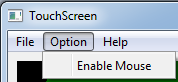
\includegraphics[width=\textwidth/3]{bilder/option-MenuBar.png}
\end{figure}\\\\
Unter File(siehe Abbildung 3.8: Start New Game) hat der Benutzer die möglichkeit das Spiel zurück zu setzten bzw. ein neues Spiel zu starten.
\begin{figure}[h]
	\centering
	\caption{Start New Game}
	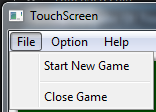
\includegraphics[width=\textwidth/3]{bilder/File-MenuBar.png}
\end{figure}\\


\cleardoublepage
%========================================================================================
% TU Dortmund, Informatik Lehrstuhl VII
%========================================================================================

\chapter{Ergebnisse}




\chapter{Diskussion}
In diesem Kapitel soll die entwickelte Lösung kritisch betrachtet werden. Dabei soll gerade auf die Schwächen der Lösung eingangen und Verbesserungsvorschläge für diese dargestellt werden.



\section{Verbesserungsvorschläge}

\subsubsection{Rendering und Physik}

\subsubsection{Kamerakalibrierung}
Die Kalibrierung der Kamera, und damit die Erkennung des gegebenen Schachbrett-/Patternmusters bzw. deren Qualität, wird sehr durch den aktuellen Lichteinfluss, u.a. durch die Einstellungen des Beamers, auf das aufgenommene Kamerabild, beeinflusst.
Sofern die genutzte Kamera nicht exakt scharf eingestellt ist oder das Bild zu dunkel oder zu hell wird, hat dies als direkte Folge eine unsaubere bzw. schlechte bis nicht funktionierende Kamera-Kalibrierung. 
Da in unserem Projekt für die Erkennung des bekannten Schachbrettmusters eine bereits existierende Methode der OpenCV-Bibliothek genutzt wurde, sind die zu optimierenden Möglichkeiten sehr eingeschränkt.
Eine lösende Variante wäre es, ein vorgefertigtes Bild anzeigen zu lassen und erst bei einem aufgenommenem Foto dieses Bildes über die Kamera, welches entsprechende Merkmale aufweist (Helligkeit, Schärfe, Ausrichtung), die Weiterleitung an die Kalibrierung zu gestatten. Somit müsste der Benutzer die Kamera und den Beamer vor der Kalibrierung bereits so einstellen, dass diese Einstellungen eine erfolgreiche Kalibrierung zufolge haben.


\subsubsection{Queue-Detektion}
Die vorgestellte Erkennung des Queues basiert stark auf der Farbe des Queues. 
Da andere Gegenstände im Kamerabild eventuell ebenfalls einen dunklen Farbton können, wäre die Erkennung in diesem Fall sehr fehleranfällig. 
Um die Erkennung robuster gegenüber diesen Störfaktoren zu machen, könnte die Erkennung des Queues auf weiteren Merkmalen, wie zum Beispiel Markern, basieren.

Weiterhin limitiert die Wiederholfrequenz der Kamera von 25 Bildern die Sekunde stark die Präzision der Steuerung. 
Durch die hohe Belichtungszeit ergibt sich eine starke Bewegungsunschärfe, gerade bei schnellen Bewegungen. 
Diese wirkt sich negativ auf die genaue Erkennung der Queue Spitze aus.
Zusätzlich sorgt die Wiederholfrequenz dafür, dass das Spiel selbst auch nur mit 25 Bildern pro Sekunde dargestellt wird. 
Anders als das erste Problem könnte dies jedoch z.B. durch ein Double-Buffering der Eingabebilder behoben werden.

Schließlich lässt sich die Modellierung des Queues an sich verbesseren.
Die Kollision basiert in der vorgestellten Lösung lediglich auf einem Punkt, der Queue-Spitze.
In der Realität hat der Queue jedoch noch eine Ausdehnung in die Breite, die bei dieser Modellierung nicht berücksichtigt wird.
% -------------------------------------------------------------------

%\cleardoublepage
%\appendix

%%========================================================================================
% TU Dortmund, Informatik Lehrstuhl VII
%========================================================================================

\chapter{Weitere Informationen}

One morning, when Gregor Samsa woke from troubled dreams, he found
himself transformed in his bed into a horrible vermin. He lay on
his armour-like back, and if he lifted his head a little he could
see his brown belly, slightly domed and divided by arches into
stiff sections. The bedding was hardly able to cover it and seemed
ready to slide off any moment. His many legs, pitifully thin
compared with the size of the rest of him, waved about helplessly
as he looked. \glqq What's happened to me?\grqq he thought. It
wasn't a dream. His room, a proper human room although a little
too small, lay peacefully between its four familiar walls. A
collection of textile samples lay spread out on the table - Samsa
was a travelling salesman - and above it there hung a picture that
he had recently cut out of an illustrated magazine and housed in a
nice, gilded frame. It showed a lady fitted out with a fur hat and
fur boa who sat upright, raising a heavy fur muff that covered the
whole of her lower arm towards the viewer. Gregor then turned to
look out the window at the dull weather. Drops of rain could be
heard hitting the pane, which made him feel quite sad.  \glqq How
about if I sleep a little bit longer and forget all this
nonsense\grqq, he thought, but that was something he was unable to
do because he was used to sleeping on his right, and in his
present state couldn't get into that position. However hard he
threw himself onto his right, he always rolled back to where he
was. He must have tried it a hundred times, shut his eyes so that
he wouldn't have to look at the floundering legs, and only stopped
when he began to feel a mild, dull pain there that he had never
felt before. \glqq Oh, God, he thought, what a strenuous career it
is that I've chosen!\grqq Travelling day in and day out. 


% -------------------------------------------------------------------

% -------------------------------------------------------------------

% Literaturverzeichnis
\addcontentsline{toc}{chapter}{Literaturverzeichnis}
\bibliographystyle{dinatls7}
\bibliography{Literatur}

% -------------------------------------------------------------------

\end{document}
